\chapter{Network Clustering}
%The network has distinct communities. In one community, Amazon is running a very convincing mass-advertising campaign. In another community there is a very convincing person. In the remaining communities nothing special is happening (there will be somewhere between 2 and 10 communities in the network). It is important to identify communities in order to do a good job.
%How did you do the community detection?
In our solution we detected communities using group based clustering.
This is the process of \textit{cutting} edges in a graph in order to split it in two subgraphs.
Each such subgraph can then be considered a cluster (possibly containing additional clusters).
We used spectral clustering to determine where to perform this \textit{cut}.
To achieve this we calculated an eigenvector decomposition using a .NET library \footnote{...}.
This decomposition is then used to determine which \textit{cut} will introduce a set of \textit{balanced} subgraphs with a minimum of change from the original graph structure (a minimum of cut edges).
Minimum is used as a vague term in this context, as it does not necessarily refer to the actual minimal change.
Instead it refers to the minimal change with respect to maintaining balance between the two subgraphs.

\section{Clusters}
The network is clustered recursively, by first defining the entire dataset as a cluster and then iteratively splitting the largest (in terms of number of people) cluster in two.
This process is repeated until the split results in one cluster with one member and another with a relatively larger number of members.

The end-result is that we have four clusters (see \cref{fig:cluster}) of sizes 683, 1167, 1750 and 619.
The clusters are represented in the same order in the figure, from top-left to bottom-right.
Their hierarchical relation is defined by the order of the splits.
The order of these split is represented in the figure as numbers and lines.

In the first and third cluster we see that one person is quite well-connected with the remaining cluster.

\begin{figure}
\centering
\begin{subfigure}[b]{0.6\textwidth}

\includegraphics[width=\linewidth]{graphics/pre-cluster}
\caption{Before clustering}
\label{fig:pre-cluster}
\end{subfigure}\\

\begin{subfigure}[b]{0.6\textwidth}
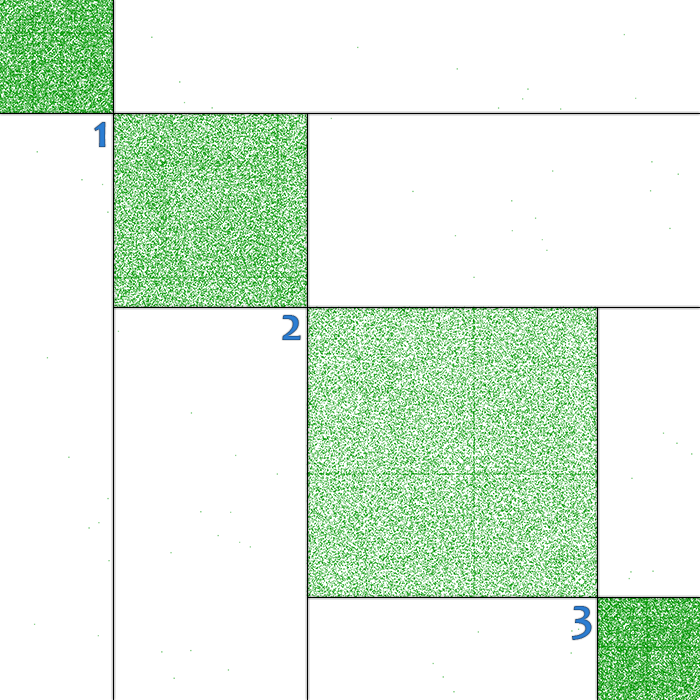
\includegraphics[width=\linewidth]{graphics/cluster}
\caption{After clustering}
\label{fig:cluster}
\end{subfigure}

\caption{Binary adjacency matrices, showing the friendship relations}
\end{figure}

%What were the results?
%Argue for you choice of algorithm or describe what you would have done, if you have had more time.

%A community “friendships.txt” file can be found in the Moodle resource folder. It should be self-explanatory (no reviews are added yet, but be ready to read in the reviews later).